\chapter{Contexte et Problematique}

\section{Introduction a la Cybersecurite Hospitaliere}

\subsection{Enjeux de la Securite dans le Secteur de la Sante}

Le secteur de la sante represente aujourd'hui l'une des cibles privilegiees des cybercriminels. Selon le rapport annuel de l'ANSSI 2024, les etablissements de sante ont subi une augmentation de 47\% des cyberattaques par rapport a l'annee precedente. Cette vulnerabilite accrue s'explique par plusieurs facteurs :

\begin{itemize}
    \item \textbf{Criticite des donnees} : Les dossiers medicaux electroniques (EMR) contiennent des informations hautement sensibles
    \item \textbf{Continuite de service} : L'impossibilite d'interrompre les soins met les hopitaux en position de faiblesse
    \item \textbf{Infrastructure complexe} : Interconnexion de systemes heterogenes (PACS, SIS, equipements biomedicaux)
    \item \textbf{Contraintes reglementaires} : Conformite RGPD, HDS, et normes de securite sanitaire
\end{itemize}

\subsection{Specificites de l'Environnement Hospitalier}

L'ecosysteme informatique hospitalier presente des caracteristiques uniques qui complexifient la mise en œuvre de solutions de securite traditionnelles :

\paragraph{Heterogeneite des Systemes}
L'infrastructure hospitaliere integre :
\begin{enumerate}
    \item \textbf{Systemes d'Information Hospitaliers (SIH)} : Gestion administrative et medicale
    \item \textbf{PACS (Picture Archiving and Communication System)} : Archivage et communication d'images medicales
    \item \textbf{Equipements biomedicaux connectes} : Moniteurs, pompes a perfusion, ventilateurs
    \item \textbf{Reseaux de telecommunication} : VoIP, systemes d'appel infirmier
    \item \textbf{Systemes de securite physique} : Controle d'acces, videosurveillance
\end{enumerate}

\paragraph{Contraintes Operationnelles}
\begin{itemize}
    \item \textbf{Disponibilite 24/7} : Aucune interruption de service acceptable
    \item \textbf{Temps de reponse critique} : Latence maximale de quelques millisecondes pour certains equipements
    \item \textbf{Mobilite du personnel} : Acces nomade et connexions multiples
    \item \textbf{Interoperabilite} : Communication entre systemes de differents editeurs
\end{itemize}

\subsection{Topologie Reseau Hospitaliere}

La figure \ref{fig:network_topology} illustre la complexite de l'architecture reseau d'un etablissement hospitalier moderne, montrant l'interconnexion des differents systemes et les flux de donnees critiques.

\begin{figure}[H]
    \centering
    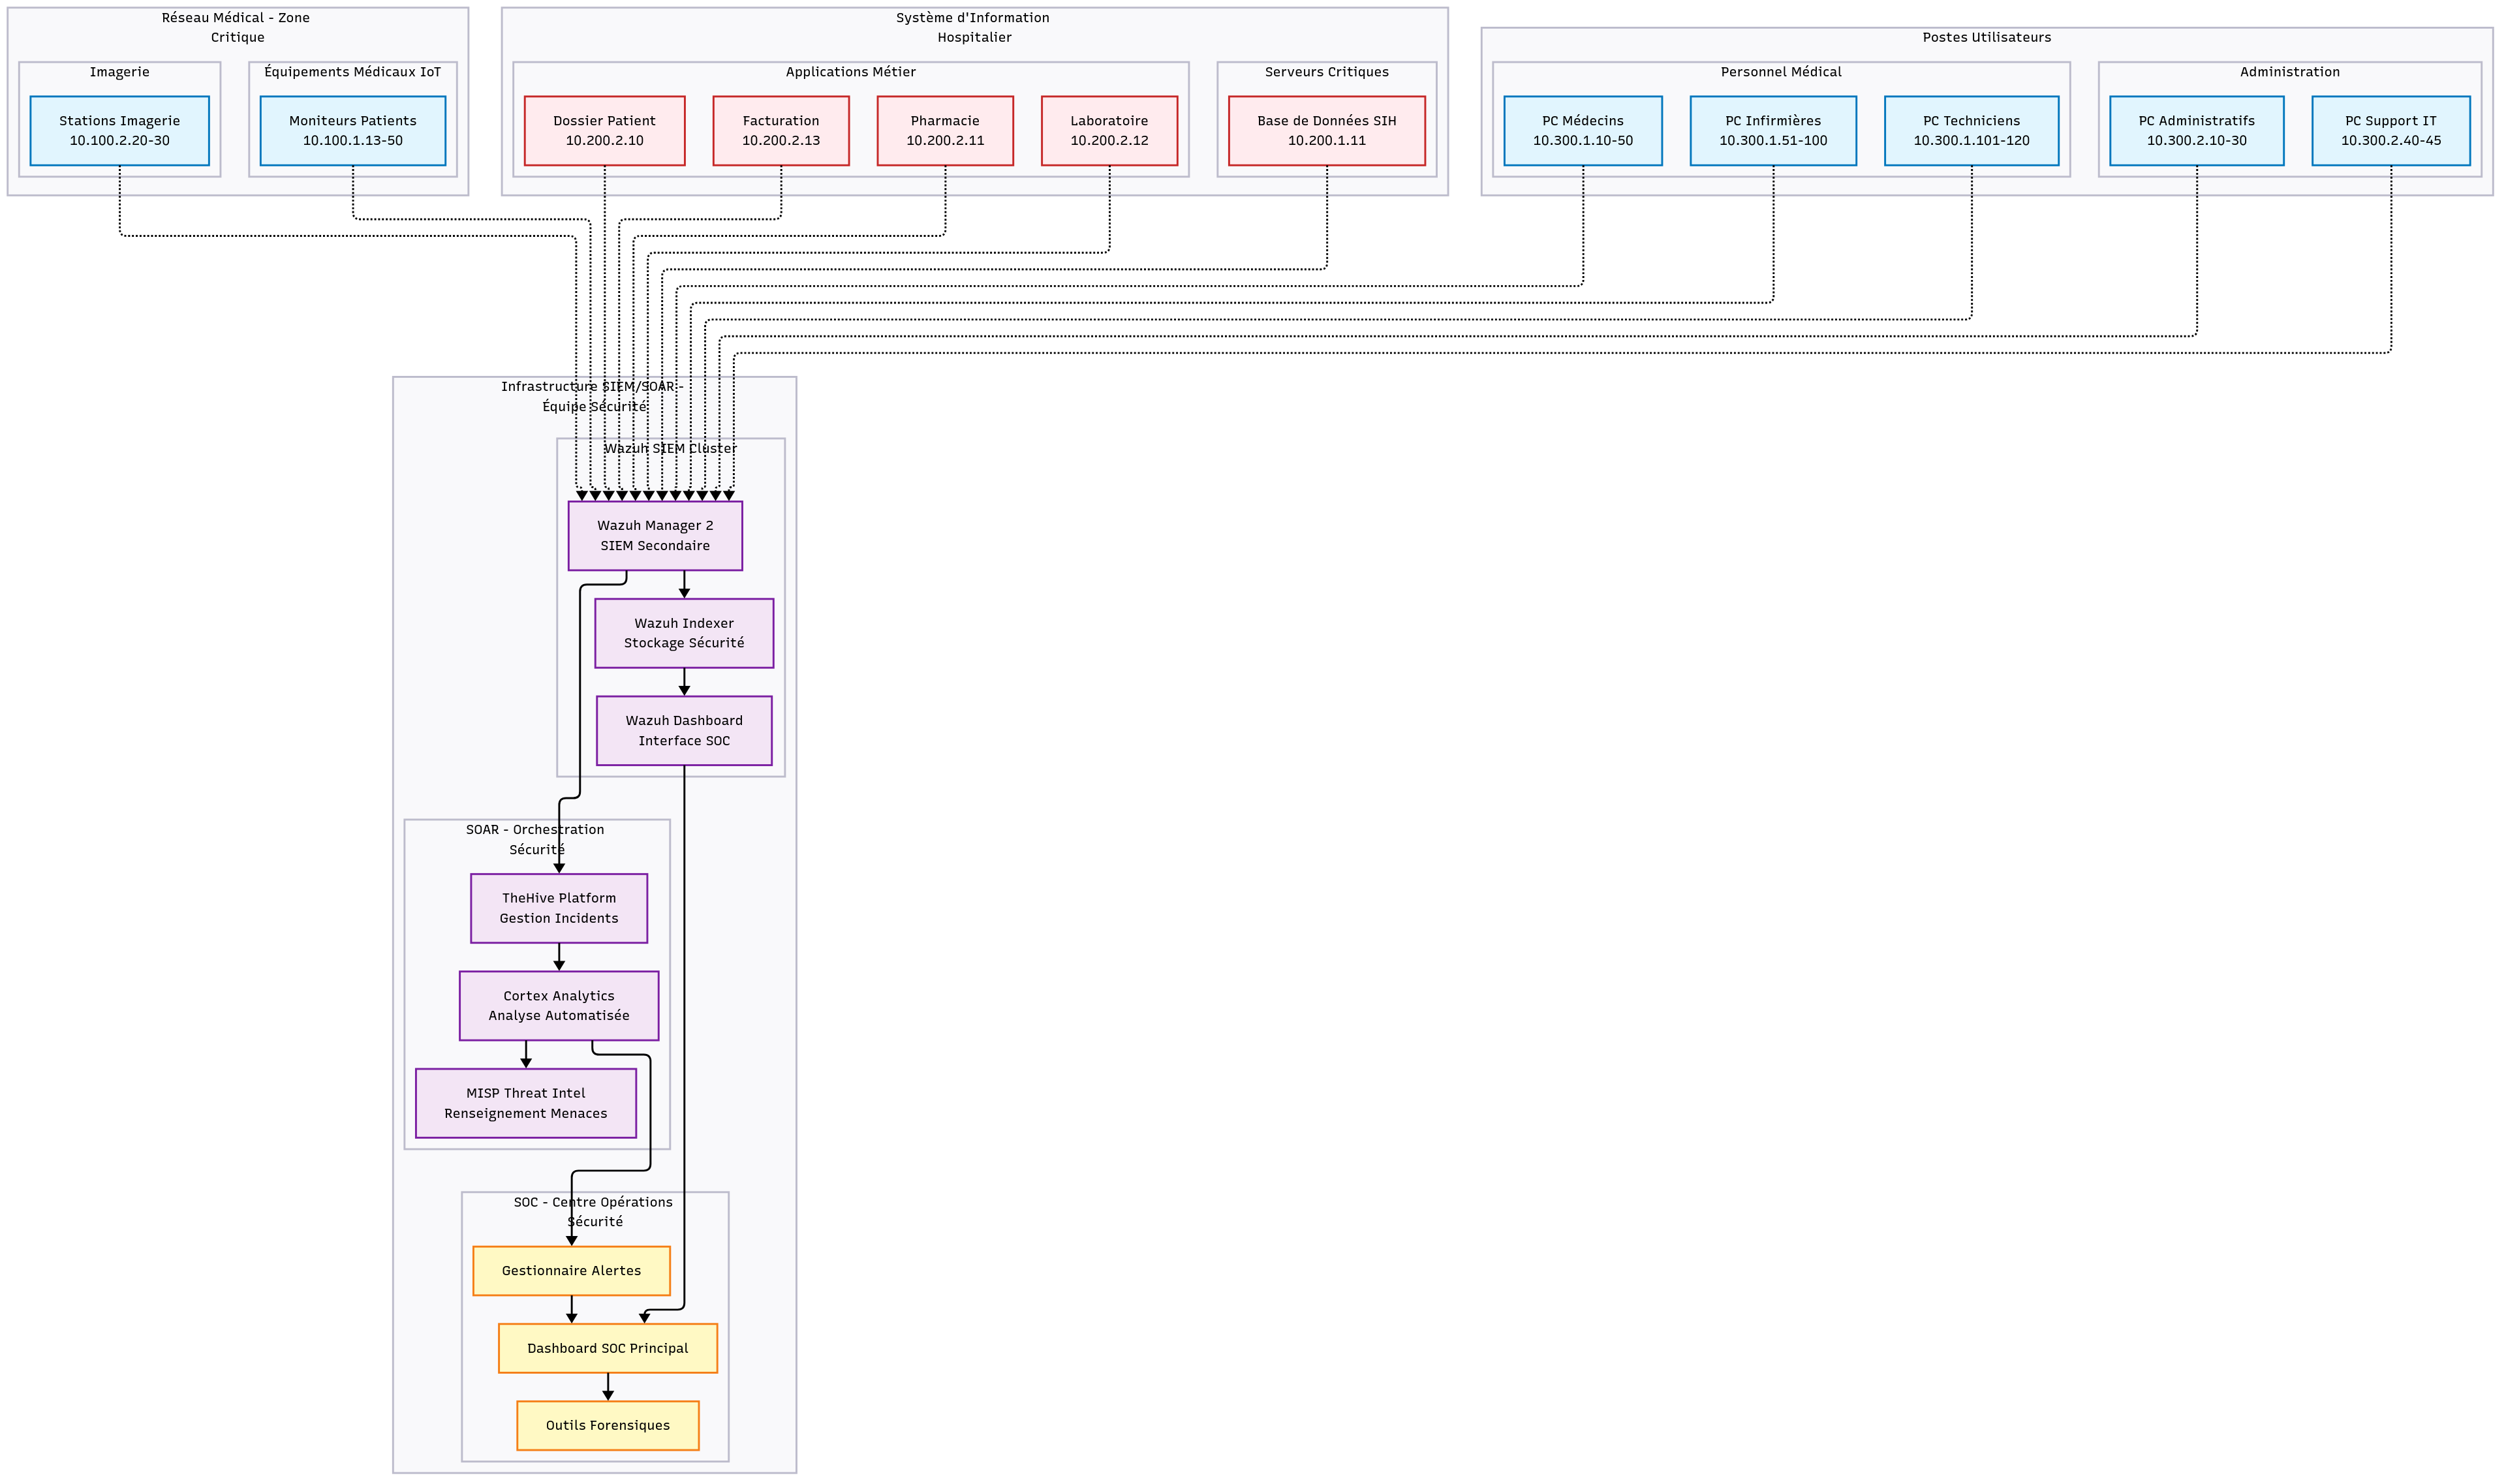
\includegraphics[width=\textwidth]{images/network_topology.png}
    \caption{Topologie reseau hospitaliere - Vue d'ensemble de l'infrastructure}
    \label{fig:network_topology}
\end{figure}

Cette architecture met en evidence les points de vulnerabilite et les zones critiques necessitant une surveillance renforcee. La segmentation reseau et la mise en place de points de controle sont essentielles pour assurer la securite de l'ensemble du systeme.

\section{Analyse des Menaces Specifiques}

\subsection{Typologie des Attaques sur les Etablissements de Sante}

\subsubsection{Ransomwares}

Les attaques par ransomware representent 67\% des incidents de securite dans le secteur hospitalier. Les variantes les plus observees incluent :

\begin{table}[H]
    \centering
    \caption{Principales familles de ransomware ciblant les hopitaux}
    \begin{tabular}{|l|l|c|l|}
        \hline
        \textbf{Famille} & \textbf{Vecteur d'Infection} & \textbf{Frequence} & \textbf{Impact Typique}    \\
        \hline
        WannaCry         & EternalBlue (SMBv1)          & 23\%               & Paralysie complete du SIH  \\
        \hline
        NotPetya         & Credential dumping           & 18\%               & Destruction de donnees     \\
        \hline
        Ryuk             & Phishing cible               & 15\%               & Chiffrement selectif       \\
        \hline
        Conti            & RDP/VPN compromise           & 12\%               & Exfiltration + chiffrement \\
        \hline
        Lockbit          & Supply chain                 & 8\%                & Attaque multi-sites        \\
        \hline
    \end{tabular}
\end{table}

\subsubsection{Compromission d'Equipements Biomedicaux}

Les equipements biomedicaux connectes presentent des vulnerabilites specifiques :

\begin{itemize}
    \item \textbf{Systemes d'exploitation obsoletes} : Windows XP/7 sans mise a jour de securite
    \item \textbf{Protocoles de communication non securises} : DICOM, HL7 sans chiffrement
    \item \textbf{Mots de passe par defaut} : Configurations d'usine non modifiees
    \item \textbf{Absence de monitoring} : Equipements isoles des systemes de surveillance
\end{itemize}

\subsection{Vecteurs d'Attaque Identifies}

L'analyse des incidents de securite dans notre environnement de test a permis d'identifier les principaux vecteurs d'attaque :

\paragraph{Attaques Reseau}
\begin{enumerate}
    \item \textbf{Exploitation de vulnerabilites SMB} : EternalBlue (MS17-010), BluekeepSafe (CVE-2019-0708)
    \item \textbf{Attaques par deni de service} : Saturation des equipements critiques
    \item \textbf{Man-in-the-middle} : Interception de communications medicales non chiffrees
    \item \textbf{Lateral movement} : Propagation horizontale apres compromission initiale
\end{enumerate}

\paragraph{Attaques Applicatives}
\begin{enumerate}
    \item \textbf{Injection SQL} : Compromission des bases de donnees patient
    \item \textbf{Cross-Site Scripting (XSS)} : Vol de sessions utilisateur
    \item \textbf{Injection de commandes} : Execution de code arbitraire
    \item \textbf{Elevation de privileges} : Compromission de comptes administrateur
\end{enumerate}

\section{Etat de l'Art des Solutions SIEM/SOAR}

\subsection{Technologies SIEM Existantes}

\subsubsection{Solutions Commerciales}

\begin{table}[H]
    \centering
    \caption{Comparaison des solutions SIEM commerciales}
    \begin{tabular}{|l|c|c|c|c|}
        \hline
        \textbf{Solution} & \textbf{EPS Max} & \textbf{Cout/GB} & \textbf{IA/ML} & \textbf{SOAR Integre} \\
        \hline
        Splunk Enterprise & 150K             & 15€              & Oui            & Phantom               \\
        \hline
        IBM QRadar        & 100K             & 12€              & Oui            & SOAR natif            \\
        \hline
        ArcSight ESM      & 75K              & 18€              & Partiel        & SOAR externe          \\
        \hline
        LogRhythm         & 50K              & 10€              & Oui            & SOAR natif            \\
        \hline
        Sentinel (Azure)  & Illimite         & 2.3€             & Oui            & Logic Apps            \\
        \hline
    \end{tabular}
\end{table}

\subsubsection{Solutions Open Source}

Les solutions open source offrent une alternative economiquement viable pour les etablissements de sante :

\begin{itemize}
    \item \textbf{Wazuh} : SIEM/XDR avec detection comportementale avancee
    \item \textbf{OSSEC} : Systeme de detection d'intrusion host-based
    \item \textbf{ELK Stack} : Elasticsearch, Logstash, Kibana pour l'analyse de logs
    \item \textbf{Graylog} : Plateforme de gestion centralisee des logs
    \item \textbf{OSSIM/AlienVault} : SIEM communautaire avec correlation de regles
\end{itemize}

\subsection{Plateformes SOAR}

\subsubsection{Orchestration et Automatisation}

Les plateformes SOAR (Security Orchestration, Automation and Response) permettent l'automatisation des processus de reponse aux incidents :

\paragraph{TheHive}
\begin{itemize}
    \item Gestion collaborative des incidents de securite
    \item Workflows personnalisables pour differents types d'alertes
    \item Integration native avec Cortex pour l'analyse automatisee
    \item API REST complete pour l'integration avec les SIEM
\end{itemize}

\paragraph{Cortex}
\begin{itemize}
    \item Plateforme d'analyse d'observables et d'artifacts
    \item Bibliotheque de plus de 100 analyzers
    \item Responders pour automatiser les actions de reponse
    \item Support des formats STIX/TAXII pour le partage de CTI
\end{itemize}

\paragraph{MISP}
\begin{itemize}
    \item Plateforme de partage de renseignement sur les menaces
    \item Base de donnees collaborative d'IOCs
    \item Taxonomies standardisees (MITRE ATT\&CK, Kill Chain)
    \item Feeds automatiques de threat intelligence
\end{itemize}

\section{Objectifs et Defis du Projet}

\subsection{Objectifs Principaux}

Ce projet vise a concevoir et implementer une solution SIEM/SOAR adaptee aux specificites de l'environnement hospitalier. Les objectifs principaux sont :

\begin{enumerate}
    \item \textbf{Detection Precoce} : Identifier les menaces dans les 5 premieres secondes
    \item \textbf{Reponse Automatisee} : Contenir 80\% des incidents sans intervention humaine
    \item \textbf{Conformite Reglementaire} : Respecter les exigences RGPD et HDS
    \item \textbf{Continuite de Service} : Maintenir la disponibilite des systemes critiques
    \item \textbf{Integration Transparente} : S'adapter a l'infrastructure existante
\end{enumerate}

\subsection{Defis Techniques Identifies}

\subsubsection{Defis d'Architecture}

\begin{itemize}
    \item \textbf{Scalabilite horizontale} : Traitement de 100K+ evenements par seconde
    \item \textbf{Haute disponibilite} : Redondance active/passive avec failover automatique
    \item \textbf{Chiffrement de bout en bout} : Protection des donnees medicales en transit
    \item \textbf{Segmentation reseau} : Isolation des environnements critiques
\end{itemize}

\subsubsection{Defis Operationnels}

\begin{itemize}
    \item \textbf{Formation du personnel} : Appropriation des outils par les equipes SOC
    \item \textbf{Tuning des regles} : Reduction du taux de faux positifs sous 5\%
    \item \textbf{Integration des processus} : Alignement avec les procedures existantes
    \item \textbf{Cout total de possession} : Optimisation des ressources et licences
\end{itemize}

\subsection{Metriques de Succes}

\begin{table}[H]
    \centering
    \caption{Indicateurs cles de performance (KPI) du projet}
    \begin{tabular}{|l|c|c|}
        \hline
        \textbf{Indicateur}       & \textbf{Valeur Cible} & \textbf{Methode de Mesure} \\
        \hline
        Temps de detection moyen  & < 30 secondes         & Monitoring automatique     \\
        \hline
        Taux de faux positifs     & < 5\%                 & Analyse hebdomadaire       \\
        \hline
        Temps de reponse incident & < 15 minutes          & Metrics TheHive            \\
        \hline
        Disponibilite systeme     & > 99.9\%              & Monitoring Nagios          \\
        \hline
        Couverture MITRE ATT\&CK  & > 80\%                & Mapping des regles         \\
        \hline
        Satisfaction utilisateur  & > 4/5                 & Enquete trimestrielle      \\
        \hline
    \end{tabular}
\end{table}

Cette premiere approche contextuelle etablit les fondements de notre projet SIEM/SOAR, en mettant en evidence les enjeux specifiques du secteur hospitalier et les defis techniques a relever.
